\chapter{The Proposed Hybrid Scheme}
\label{sec:hybrid}

This chapter describes the design and the components of our \hybrid. In \Cref{sec:hybrid.structure} we provide an overview of our \hybrid, in \Cref{sec:hybrid.scheme} we describe the \erbac, and in \Cref{sec:hybrid.cac} we describe the \cac modified according to our \erbac. %, and in \Cref{sec:hybird_istantiation} we provide an example an istantiation of our extended model.

\section{High-Level Structure of the \Hybrid}
\label{sec:hybrid.structure}

% \begin{figure}[t]
%     \centering
%     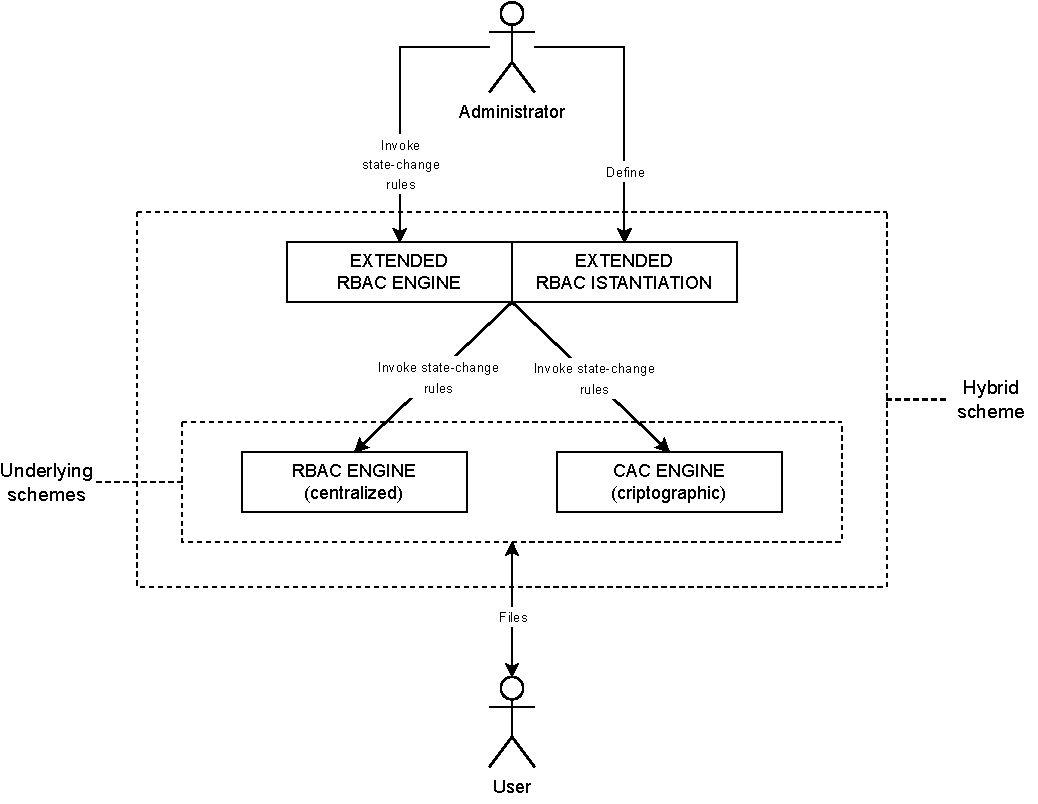
\includegraphics[width=0.75\textwidth]{assets/img/hybrid_scheme.pdf}
%     \caption{\label{fig:hybrid_scheme}The hybrid scheme}
% \end{figure}

Security models typically assume that the \gls{csp} is either completely trusted or honest-but-curious. However, in practice, the actual situation is often somewhere in between, which can allow for more efficient operations and a reduced amount of cryptographic computations. To the best of our knowledge, there is no \gls{ac} \erbacwhat in the literature allowing administrators to specify the security model for their scenario. To this end, we provide an extended \gls{rbac} scheme.
At a high level, the \erbac is automatically compiled into a \centralized and a \cac. The \centralized can be enforced by a traditional \gls{rbac} enforcement mechanisms (e.g., those provided directly by \glspl{csp}). The \cac, as proposed in \cite{cac}, is not able to handle a dynamic security model (e.g., it is not always necessary to re-encrypt a file), so it is necessary to make the changes described in \Cref{sec:background.cac}. The administrator operates on the extended \gls{rbac} model by invoking its state-change rules, which in turn invoke the state-change rules of the centralized \gls{ac} and \gls{cac}, so that enforcement is performed only by these two mechanisms.
To define the security model, we define the concept of predicate, introduce new queries, and modify the entailment as described below.

\paragraph{Predicates.} Predicates are facts, characteristics, or requirements related to users, files, or the \gls{csp}. Predicates are dependent on company processes. For example, if files have different levels of sensitivity, the administrator can introduce a predicate for each level. This results in \( \function{topSecret}(\file) \) for top secret files, \( \function{secret}(\file) \) for secret files, and \( \function{public}(\file) \) for public files. Another example is a company where employees have a smart card that contains the keys \( \keysigu \) and \( \keydecu \) for \gls{cac}, the administrator might want to model the case where the card is lost and all files need to be re-encrypted. To achieve this, a \( \function{lostKeyCard}(\user) \) predicate could be introduced. Our proposal only supports unary predicates, which are predicates applied to a single entity. Although it is possible to introduce predicates on more than one entity, we chose to maintain greater simplicity by only supporting unary predicates.

\paragraph{Queries.} There are several aspects of \gls{cac} that can be customized, and to control each one, new queries were introduced in the \erbac. These queries serve as the interface between the \erbac and the administrator's chosen security model. For instance, the \( \isEncryptionNeededQ \) query determines whether a file should be encrypted or not. \Cref{sec:hybrid.scheme} provides a detailed discussion of queries and their meanings. 


\paragraph{Entailment Instantiation.} The instantiation of the entailment function should result in a \( \mathit{true} \) or \( \mathit{false} \) answer when called with one of the new queries. The answer may be dependent on the predicate assignment. For instance, if a \( \function{confidential} \) predicate exists, the entailment function is instantiated so that when a file \( \file \) has the \( \function{confidential}(\file) \) predicate, the entailment function called with \( \isEncryptionNeededQ \) returns \( \mathit{true} \); \( \mathit{false} \) otherwise.

\Cref{fig:hybrid_structure} illustrates the operations performed in the \hybrid. Specifically, \Cref{fig:hybrid_structure.admin} describes the process an administrator follows when invoking a state-change rule. The proxy receives the invocation and retrieves metadata, including predicates, from the metadata manager. As a result of the execution of the state-change rule --- and according to the retreived metadata --- the proxy updates the centralized \gls{ac} policy and metadata in the metadata manager to reflect the changes in the policy. Finally, it encrypts or decrypts any files for which the protection enforcement mechanism has been altered. \Cref{fig:hybrid_structure.read} illustrates a user reading a file. The user sends a request to the proxy, which retrieves metadata from the metadata manager. The proxy then requests the file from the data manager, which in turn consults the centralized \gls{rbac} mechanism to determine if it can send the file to the user. If authorized, the proxy receives the file and delivers it to the user, decrypting it if necessary. Finally, in \Cref{fig:hybrid_structure.write}, a user writes a file. The plaintext file is sent to the proxy, which retrieves the metadata and determines whether to encrypt the file. If encryption is necessary, the proxy encrypts the file and sends it, along with the new metadata, to the reference monitor. Firstly, the reference monitor retrieves metadata from the metadata manager. Secondly, the reference monitor verifies that the data received from the user is well-formed, checks if the user has permission to write, and ensures that the metadata is consistent. If everything is in order, the metadata is written and the new data is sent to the data manager. The data manager then verifies with the centralized RBAC mechanism whether the user is authorized to write the file. If authorized, the file is written.

% \stefanonote{Non sarebbe male discutere un attimo le figure 3.1a, 3.1b, e 3.1c --- nel senso, spiegare brevemente gli step che vengono effettuati richiamando i concetti introdotti alla fine della Sezione 2.2 (poi non mi sembra diciamo cos'è l'Access Controller; forse meglio rimpiazzare ``Access Controller'' con ``Traditional/Centralized RBAC Enforcement Mechanisms'' o qualcosa di simile?)}


\begin{figure}[t!]
    \centering

    \begin{subfigure}{\textwidth}
        \centering
        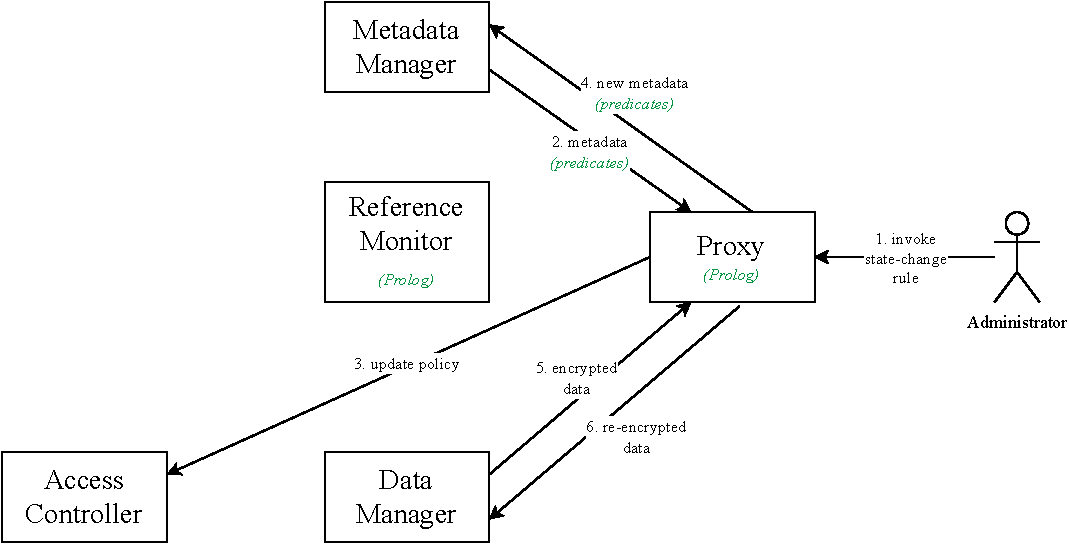
\includegraphics[width=0.7\textwidth]{assets/img2/hybrid_admin.pdf}
        \caption{State-change rule invocation}
        \label{fig:hybrid_structure.admin}
    \end{subfigure}
    \par\bigskip
    \begin{subfigure}{\textwidth}
        \centering
        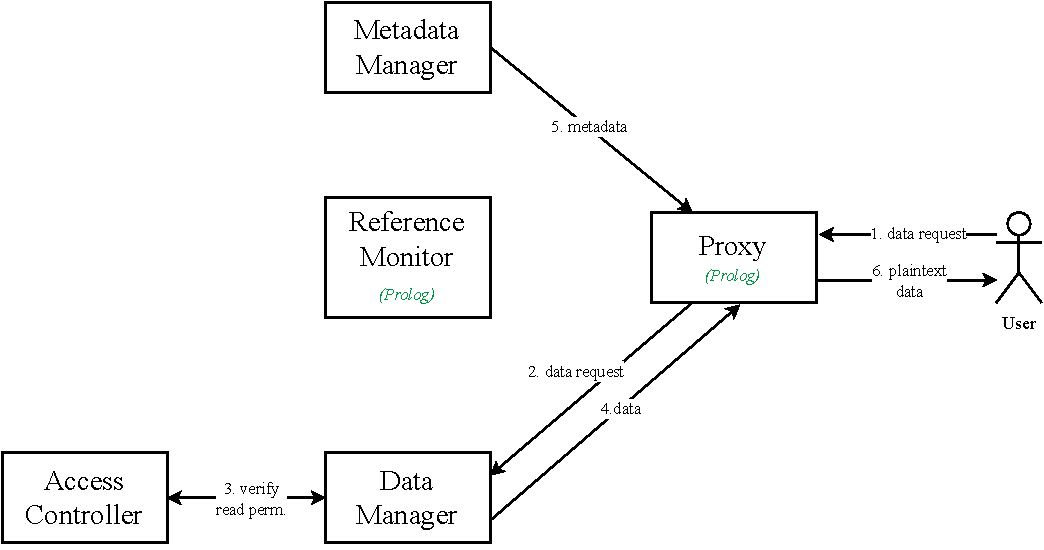
\includegraphics[width=0.7\textwidth]{assets/img2/hybrid_read.pdf}
        \caption{File reading}
        \label{fig:hybrid_structure.read}
    \end{subfigure}
    \par\bigskip
    \begin{subfigure}{\textwidth}
        \centering
        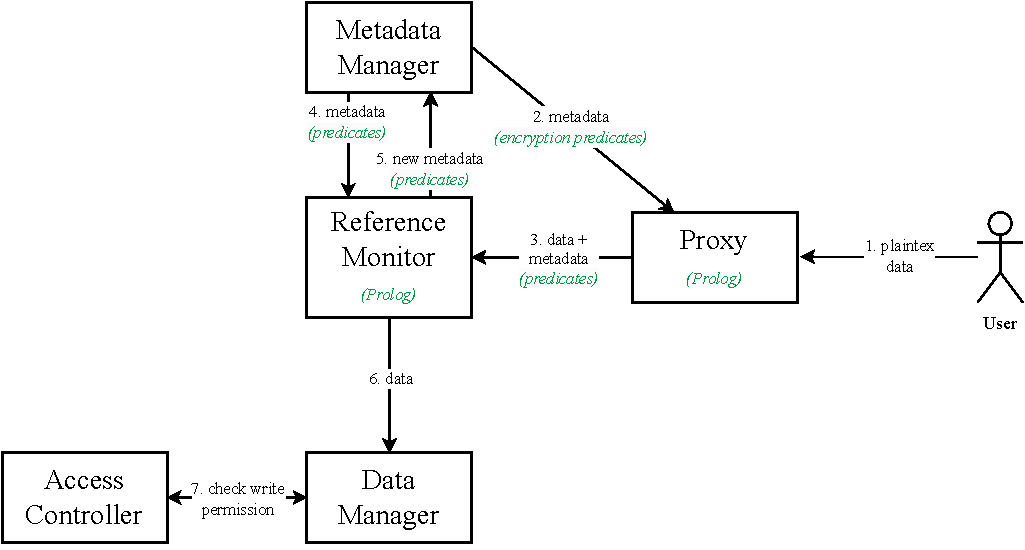
\includegraphics[width=0.7\textwidth]{assets/img2/hybrid_write.pdf}
        \caption{File writing}
        \label{fig:hybrid_structure.write}
    \end{subfigure}

    \caption{Operations In Hybrid Scheme}
    \label{fig:hybrid_structure}
\end{figure}


\section{The Extended Role-Based Access Control Scheme}
\label{sec:hybrid.scheme}

To support security model handling in the extended \gls{rbac} model, we introduce a set of predicates, assign predicates to entities, add new queries, and redefine the entailment function. 

Predicates are defined by the administrator based on the needs of the company. To enable this, a new set of predicates \( \predicates \) was introduced, with each predicate being represented as a string. As a result, the state transition system is redefined by adding the set \( \predicates \), resulting in the system being represented as \( \angular{\states, \queries, \entailment, \scrules, \predicates} \). Predicates are applied to an entity (i.e., user, role, the \gls{csp}), and they are unary. A new set, \( \prassignement \), was introduced to store the assignment. \( \prassignement \) is defined as \( \prassignement \subseteq \predicates \times (\users \cup \roles \cup \files) \). Consequently, the state was extended to also contain the set \( \prassignement \), resulting in \( \angular{\users, \roles, \files, \urassignement, \frassignement, \prassignement} \). New queries have been added to the set of queries \( \queries \), on top of the already existing \( \canDoQ \) query. Each query adjusts a specific tunable aspect of the system, such as whether to encrypt a file or not, and whether to re-encrypt a file. \Cref{tab:hybrid_queries} describes the queries, which are not customizable by the administrator. The entailment function \( \entailment \) serves as the connection between company phenomenons (the predicates) and customizable features (the queries). It is necessary for the administrator to define the entailment function for new queries based on the chosen security model. 

Note that the administrator cannot modify the entailment function for the query \( \canDoQ \), as doing so would prevent the use of a centralized \gls{rbac} and \gls{cac} mechanism. Additionally, modifying the \( \canDoQ \) query would result in a model that is no longer \gls{rbac}.

\Cref{fig:exrbac_components} illustrates the predicates, queries, and entailment function, and distinguishes between the \erbac and the security model.

\Cref{sec:hybird_istantiation} contains an example of a realistic security model instantiation.

\begin{figure}[t!]
	\centering
	
	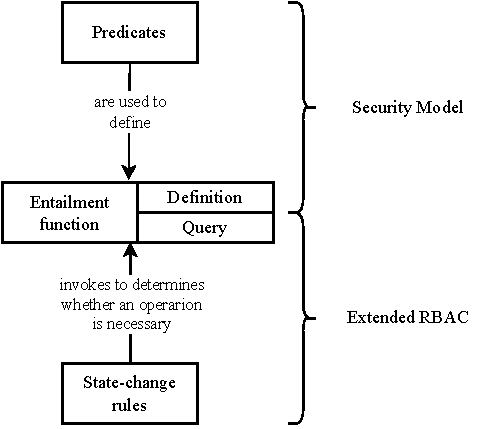
\includegraphics[width=0.5\textwidth]{assets/img2/security_model.pdf}
	
	\caption{The Interaction Between Components}
	\label{fig:exrbac_components}
\end{figure}


\wraptable{|l|X|}{\label{tab:hybrid_queries}The \( \queries \) of the hybrid model}{
	\twocols{\tabletitle{Query}}
	{\tabletitle{Description}}
	\twocols{\( \canDoQ \)}
	{Determines whether user \( \user \) has access to file \( \file \) to perform the action \( \operation \)}
	\twocols{\( \isEncryptionNeededQ \)}
	{Determines whether it is necessary to encrypt the file \( \file \)}
	\twocols{\( \isReencryptionNeededOnRPQ \)}
	{Determines whether it is necessary to re-encrypt the file \( \file \) when the permission \( \angular{\operation, \file} \) is revoked}
	\twocols{\( \isEagerReencNeededOnRPQ \)}
	{Determines whether it is necessary immediately to re-encrypt the file \( \file \) when the permission \( \angular{\operation, \file} \) is revoked}
	\twocols{\( \isRoleKeyRotationNeededOnRURQ \)}
	{Determines whether it is necessary to rotate the key of role \( \role \) when 
		the membership of the user \( \user \) to the role \( \role \) is revoked}
	\twocols{\( \isReencryptionNeededOnRURQ \)}
	{Determines whether it is necessary to re-encrypt the file \( \file \) when the membership of the user \( \user \) to the role \( \role \) is revoked}
	\twocols{\( \isEagerReencNeededOnRURQ \)}
	{Determines whether it is necessary to re-encrypt immediately the file \( \file \) when the membership of the user \( \user \) to the role \( \role \) is revoked}
}

\pagelisting{\label{list:extended_changestate}The state-change rules \( \scrules \) of the hybrid model }{\scriptsize}{b!}{
    \begin{itemize}

        %% --- addUser ---
        \item \( \addUserF \)
        \begin{itemize}
            \item Update state with \( \statete{\users \cup \setof{\user}}{\roles}{\files}{\urassignement}{\frassignement}{\prassignement} \)
            \item \( \addUserFC \)
            \item \( \addUserFK \)
        \end{itemize}

        %% --- deleteUser ---
        \item \( \deleteUserF \)
        \begin{itemize}
            \item Update state with \( \statete{\users \setminus \setof{\user}}{\roles}{\files}{\urassignement}{\frassignement}{\prassignement} \)
            \item For each \( (\user, \role) \in \urassignement \):
            \begin{itemize}
                \item \( \revokeUserFromRoleFC \)
                \item \( \revokeUserFromRoleFK \)
            \end{itemize}
            \item \( \deleteUserFC \)
            \item \( \deleteUserFK \)
        \end{itemize}

        %% --- addRole ---
        \item \( \addRoleF \)
        \begin{itemize}
            \item Update state with \( \statete{\users}{\roles \cup \setof{\role}}{\files}{\urassignement}{\frassignement}{\prassignement} \)
            \item \( \addRoleFC \)
            \item \( \addRoleFK \)
        \end{itemize}

        %% --- deleteRole ---
        \item \( \deleteRoleF \)
        \begin{itemize}
            \item Update state with \( \statete{\users}{\roles \setminus \setof{\role}}{\files}{\urassignement}{\frassignement}{\prassignement} \)
            \item For each \( (\role, \twoang{\operation}{\file}) \in \frassignement \):
            \begin{itemize}
                \item \( \revokePermissionFromRoleF \)
            \end{itemize}
            \item \( \deleteRoleFC \)
            \item \( \deleteRoleFK \)
        \end{itemize}

        %% --- addResource ---
        \item \( \addResourceF \)
        \begin{itemize}
            \item Update state with \( \statete{\users}{\roles}{\files \cup \setof{\file}}{\urassignement}{\frassignement}{\prassignement} \)
            \item \( \addResourceFC \)
        \end{itemize}

        %% --- deleteResource ---
        \item \( \deleteResourceF \)
        \begin{itemize}
            \item Update state with \( \statete{\users}{\roles}{\files \setminus \setof{\file}}{\urassignement}{\frassignement}{\prassignement} \)
            \item \( \deleteResourceFC \)
            \item For each \( (\role, \twoang{\operation}{\file}) \in \frassignement \):
            \begin{itemize}
                \item \( \revokePermissionFromRoleF \)
            \end{itemize}
            \item If \( \isEncryptionNeededF \):
            \begin{itemize}
                \item \( \deleteResourceFK \)
            \end{itemize}
        \end{itemize}

        %% --- assignUserToRole ---
        \item \( \assignUserToRoleF \)
        \begin{itemize}
            \item Update state with \( \statete{\users}{\roles}{\files}{\urassignement \cup \setof{(\user, \role)}}{\frassignement}{\prassignement} \)
            \item \( \assignUserToRoleFC \)
            \item \( \assignUserToRoleFK \)
        \end{itemize}

        %% --- assignPermissionToRole ---
        \item \( \assignPermissionToRoleF \)
        \begin{itemize}
            \item Update state with \( \statete{\users}{\roles}{\files}{\urassignement}{\frassignement \cup (\role, \twoang{\operation}{\file})}{\prassignement} \)
            \item \( \assignPermissionToRoleFC \)
            \item If \( \isEncryptionNeededF \):
            \begin{itemize}
                \item \( \assignPermissionToRoleFK \)
            \end{itemize}
        \end{itemize}

    \end{itemize}
}{
    \begin{itemize}

        %% --- revokeUserFromRole ---
        \item \( \revokeUserFromRoleF \)
        \begin{itemize}
            \item \( \revokeUserFromRoleFC \)
            \item For each \( (r, \twoang{\operation}{\file}) \in \frassignement \) with \( \isEncryptionNeededF \)
            \begin{itemize}
                \item \( \revokeUserFromRoleFK \)
                \item If \( \isReencryptionNeededOnRURF \):
                \begin{itemize}
                    \item \( \prepareReencryptionF \)
                \end{itemize}
                \item If \( \isEagerReencNeededOnRURF \):
                \begin{itemize}
                    \item \( \reencryptResourceF \)
                \end{itemize}
            \end{itemize}
            \item \( \revokeUserFromRoleFK \)
            \item If exists \( (r, \twoang{-}{\file}) \in \frassignement \) with \( \isEncryptionNeededF \) and \( \isRoleKeyRotationNeededOnRURF \):
            \begin{itemize}
                \item \( \rotateRoleKeyF \)
            \end{itemize}
            \item Update state with \( \statete{\users}{\roles}{\files}{\urassignement \setminus \setof{(\user, \role)}}{\frassignement}{\prassignement} \)
        \end{itemize}

        %% --- revokePermissionFromRole ---
        \item \( \revokePermissionFromRoleF \)
        \begin{itemize}
            \item \( \revokePermissionFromRoleFC \)
            \item If \( \isEncryptionNeededF \):
            \begin{itemize}
                \item \( \revokePermissionFromRoleFK \)
                \item If \( \isReencryptionNeededOnRPF \):
                \begin{itemize}
                    \item \( \prepareReencryptionF \)
                \end{itemize}
                \item If \( \isEagerReencNeededOnRPF \):
                \begin{itemize}
                    \item \( \reencryptResourceF \)
                \end{itemize}
            \end{itemize}
            \item Update state with \( \statete{\users}{\roles}{\files}{\urassignement}{\frassignement \setminus (\role, \twoang{\operation}{\file})}{\prassignement} \)
        \end{itemize}

        %% --- updateEncryptedFiles ---
        \item \( \updateEncryptedFilesF \)
        \begin{itemize}
            \item For each \( \file \in (file_1 \setminus file_2) \):
            \begin{itemize}
                \item For each \( (\role, \twoang{\operation}{\file}) \in \prassignement \):
                \begin{itemize}
                    \item \( \revokePermissionFromRoleFK \)
                \end{itemize}
                \item \( \deleteResourceFK \)
            \end{itemize}
            \item For each \( \file \in (file_2 \setminus file_1) \):
            \begin{itemize}
                \item \( \addResourceFK \)
                \item For each \( (r, \twoang{\operation}{\file}) \in \prassignement \):
                \begin{itemize}
                    \item \( \assignPermissionToRoleFK \)
                \end{itemize}
            \end{itemize}
        \end{itemize}

        %% --- assignPredicate ---
        \item \( \assignPredicateF \)
        \begin{itemize}
            \item Set \( files_1 \leftarrow \setof{\file \in \files \vert \isEncryptionNeededF} \)
            \item Update state with \( \statete{\users}{\roles}{\files}{\urassignement}{\frassignement}{\prassignement \cup \setof{\predicate, \actor}} \)
            \item Set \( files_2 \leftarrow \setof{\file \in \files \vert \isEncryptionNeededF} \)
            \item \( \updateEncryptedFilesF \)
        \end{itemize}

        %% --- revokePredicate ---
        \item \( \revokePredicateF \)
        \begin{itemize}
            \item Set \( files_1 \leftarrow \setof{\file \in \files \vert \isEncryptionNeededF} \)
            \item Update state with \( \statete{\users}{\roles}{\files}{\urassignement}{\frassignement}{\prassignement \setminus \setof{\predicate, \actor}} \)
            \item Set \( files_2 \leftarrow \setof{\file \in \files \vert \isEncryptionNeededF} \)
            \item \( \updateEncryptedFilesF \)
        \end{itemize}


    \end{itemize}
}


% \stefanonoter{I feel that in this section we present to the reader the extensions we made to RBAC but do not really explain them or the underlying motivations. Even though (extremely) difficult for us, we should always keep in mind that the reader is generally knowledgeable but knows nothing of our work --- everything we do should be motivated and explained. For instance, it is not sufficient to say that ``The set of queries is shown in \Cref{tab:hybrid_queries}.'', we should also describe/explain them. The same reasoning applies to the set of state-change rules in \Cref{list:extended_changestate}}
\section{The Modified Cryptographic Access Control Scheme}
\label{sec:hybrid.cac}

The scheme proposed in \cite{cac} assumes a specific security model. For example, it assumes that the \gls{csp} is honest-but-curious and therefore not trusted to protect any files. It also assumes that users could always collude with the \gls{csp}. Based on the previous security model, the scheme determines which operation to perform, resulting in many computationally expensive operations, such as always re-encrypting all files. To compile the security model chosen by the administrator in \gls{cac}, modifications are required. The changes can be categorized into two groups: isolating specific instructions, such as separating the revocation part of a permission from the re-encryption of files that a user previously had access to, and implementing functionality that was not originally provided, such as the ability to perform eager re-encryption.

The purpose of the changes is to ensure the following characteristics:
\begin{itemize}
	\item \textbf{role key rotation}: the original \cacwhat assumes that a user can save the role key and continue to use it even if access is revoked, so the keys are always changed when a revocation occurs. Not all security models provide for this, so it's necessary to make this operation optional;
	
	\item \textbf{file re-encryption}: whenever a permission is revoked or a user is revoked from a role, the file is re-encrypted. This operation may not be necessary (e.g. because a user has been promoted to another role and is considered trusted). Re-encryption should be separate from revocation and should be optional;
	
	\item \textbf{eager/lazy re-encryption}: the original scheme only implements lazy re-encryption, meaning that each time a file is re-encrypted, a new key and corresponding tuples are generated. However, the file is not actually re-encrypted until the first write, which improves performance. There is no mention of eager re-encryption in the original scheme. However, it is intended to allow for eager re-encryption, where a file can be re-encrypted immediately, or lazy re-encryption, where it is re-encrypted at the first write, from time to time.
\end{itemize}

To achieve the features described above, the state-change rule has been modified as follows. \( \deleteUserFK \) now only checks that the user is no longer assigned to a role. \( \deleteResourceFK \) now simply checks that no associated permissions exist and deletes the file tuple. \( \deleteRoleFK \) now simply checks that no user is assigned to role \( \role \) and that no file has a permission associated with \( \role \). The state-change rules \( \revokeUserFromRoleFK \) and \( \revokePermissionFromRoleFK \) have been modified to exclude the part that re-encrypts files. This part has been moved to a separate state-change rule called \( \prepareReencryptionF \), which prepares the file for re-encryption. A state-change rule \( \reencryptResourceF \) has been introduced to immediately re-encrypt a pending file. To achieve lazy re-encryption, it is sufficient to call \( \prepareReencryptionF \). For eager re-encryption, it is also necessary to call \( \reencryptResourceF \) immediately afterward. The part that regenerates the role key \( \role \) in the state-change rule \( \revokeUserFromRoleFK \) was removed. This part was moved to a separate state-change rule called \( \rotateRoleKeyF \). The outcome can be found in \Cref{list:cac_reimpl}.

% Thirdly, eager re-encryption expects the file to be reencrypted immediately when re-encryption is triggered (e.g. because a user loses access), whereas lazy re-encryption expects it to be reencrypted when it is first written \stefanonote{Could we perhaps explain more in detail what ``lazy'' re-encryption is? that is, the current version of the file is left as it is --- i.e., encrypted with the old sym key --- while future versions of the file will be encrypted by users with the new sym key}. The proposal in \cite{cac} provides only lazy re-encryption for reasons of efficiency; some files may be sensitive and it is necessary to reencrypt them immediately. The modified system allows one to choose on a case-by-case basis whether to do eager or lazy re-encryption. As a result, the scheme was modified in two ways: certain operations were made executable only under specific conditions, and certain operations were isolated for individual execution. 

% For instance, \Cref{list:refactor_code} illustrates the function before and after our modifications; in fact, \newline \( \revokeUserFromRoleF \) removes the tuple that allows the user to decrypt the role key, rotates the role key, and prepares the files to be re-encrypted on first access. \Cref{list:cac_reimpl} shows the outcome of all the following changes:
% \begin{itemize}
	%     \item \( \function{revokeU}(\user, \role) \): it no longer rotates the role key and does not re-encrypt files for which access is lost;
	%     \item \( \function{revokeP}(\role, \angular{\file, \operation}) \): it no longer re-encrypt files for which access is lost;
	%     \item a function called \( \function{rotateR}(\role) \) has been introduced, which rotates the key of role \( \role \);
	%     \item a function called \( \function{prepareReenctyption}(\file) \) has been introduced, which creates tuples for lazy-re-encryption;
	%     \item a function called \( \function{reencryptResource}(\file) \) has been introduced, which reencrypt the file is a lazy-encryption is pending.
	% \end{itemize}


% \stefanonote{So we want to say that the CAC scheme by Garrison et al. specifies the implementation of RBAC state-change rules for CAC {\bf but} such an implementation expects some RBAC state-change rules to execute multiple cryptographic computations, our point being that some of these cryptographic computations may not need to be executed according to the specified predicates, therefore in \Cref{list:extended_changestate,list:cac_reimpl} we identify and highlight ``atomic'' cryptographic computations and make the execution of such atomic cryptographic computations conditional/dependent on queries/predicates?}


\pagelisting{\label{list:cac_reimpl} \gls{cac} scheme \cite{cac} modified}{\ssmall}{p}{
    \begin{itemize}

        % --- AddUser ---
        \item \( \addUserFK \)
        \begin{itemize}
            \item User \( \user \) generate encryption key pair \( \keyencpairu \leftarrow \genpub \) and signature key pair \( \keysigpairu \leftarrow \gensig \)
            \item User \( \user \) sends \( \keyencu \), \( \keyveru \) to admin 
            \item Admin adds \( (\user, \keyencu, \keyveru) \) to USERS
        \end{itemize}

        % --- deleteUser ---
        \item \( \deleteUserFK \)
        \begin{itemize}
            \item Verifies that there are no tuples \rt{u}{-}{-}{sig} \verification{with \verifysig{\keyver{SU}}{\rts{u}{-}{-}, sig}}
        \end{itemize}

        % --- addResource ---
        \item \( \function{addResourceK}(\user, \file) \)
        \begin{itemize}
            \item Generate symmetric key \( \keyn \leftarrow \gensym \)
            \item Send \( \ft{\file.\fname}{1}{\encsym{k}{\file.\fcontent}}{\user}{\sig{u}} \) and \( \pt{SU}{\twoang{\file.\fname}{ \opreadwrite}}{1}{\encpub{\keyenc{SU}}{k}}{u}{\sig{u}} \) to R.M.
            \item The R.M. receives \( \ft{fn}{1}{c}{u}{sig} \) and \( \pt{SU}{\twoang{fn}{\opreadwrite}}{1}{c'}{u}{sig'} \) \verification{and verifies that the tuple are well-formed and the signatures are valid, i.e., \( \verifysig{\keyveru}{\fts{fn}{1}{c}{u}, sig} \) and \( \verifysig{\keyveru}{\pts{SU}{\twoang{fn}{\opreadwrite}}{1}{c'}{u}, sig'} \)}
            \item \verification{If verifications is successful, t}\noverification{T}he R.M. adds \( (\file.\fname,1) \) to FILES and stores \( \ft{fn}{1}{c}{u}{sig} \) and \( \pt{SU}{\twoang{fn}{\opreadwrite}}{1}{c'}{u}{sig'} \) 
        \end{itemize}

        % --- deleteResource ---
        \item \( \deleteResourceFK \)
        \begin{itemize}
            \item Verifies that there are no tuples \pt{-}{\twoang{\file.\fname}{-}}{-}{-}{-}{sig} \verification{with \verifysig{\keyver{SU}}{\pts{-}{\twoang{\file.\fname}{-}}{-}{-}{-}, sig}}
            \item Remove \( (\file.\fname, v_{\file.\fname}) \) from FILES
            \item Delete \( \ft{\file.\fname}{-}{-}{-}{-} \)
        \end{itemize}

        % --- addRole ---
        \item \( \addRoleFK \)
        \begin{itemize}
            \item Generate encryption key pair \( \keyencpairr{1} \leftarrow \genpub \) and \( \keysigpairr{1} \leftarrow \gensig \)
            \item Add \( (r, 1, \keyencr{1}, \keyverr{1}) \) to ROLES
            \item Send \( \rt{SU}{(r, 1)}{\encpub{\keyenc{SU}}{\keydecr{1}, \keysigr{1}}}{\sig{SU}} \) to R.M.
        \end{itemize}

        % --- deleteRole ---
        \item \( \deleteRoleFK \)
        \begin{itemize}
            \item Verifies that there are no tuples \pt{(\role, -)}{-}{-}{-}{-}{sig} \verification{with \verifysig{\keyver{SU}}{\pts{(\role, -)}{-}{-}{-}{-}, sig}}
            \item Verifies that there are no tuples \rt{-}{(\role, -)}{-}{sig} \verification{with \verifysig{\keyver{SU}}{\rts{-}{(\role, -)}{-}, sig}}
            \item Remove \( (\role, \rolev, -, -) \) from ROLES
        \end{itemize}

        % --- assignUserToRole ---
        \item \( \assignUserToRoleFK \)
        \begin{itemize}
            \item Find \( \rt{SU}{(\role, \rolev)}{c}{sig} \) with \( \verifysig{\keyver{SU}}{\rts{SU}{(\role, \rolev)}{c},sig} \)
            \item Decrypt keys \( (\keydecr{\rolev}, \keysigr{\rolev}) = \decpub{\keydec{SU}}{c} \)
            \item Send \( \rt{\user}{(\role, \rolev)}{\encpub{\keyencu}{\keydecr{\rolev}, \keysigr{\rolev}}}{\keyveru} \) to R.M.
        \end{itemize}

        % --- rotateRoleKey ---
        \item \( \rotateRoleKeyF \)
        \begin{itemize}
            \item Generate new role key \( (\keyencr{\rolev+1}, \keydecr{\rolev + 1}) \leftarrow \genpub \) and \( \keysigpairr{\rolev+1} \leftarrow \gensig \)
            \item For all \( \rt{u}{(\role, \rolev)}{c}{sig} \)\verification{ and \( \verifysig{\keyver{SU}}{\rts{u}{(\role, \rolev)}{c}, sig} \)}:
            \begin{itemize}
                \item Send \( \rt{u}{(\role, \rolev+1)}{\encpub{\keyenc{u}}{\keydecr{\rolev+1}, \keysigr{\rolev+1}}}{\sig{SU}} \) to R.M.
            \end{itemize}

            \item For every \( fn \) such that there exists \( \pt{(\role, \rolev)}{\twoang{fn}{\operation}}{\filev}{c}{SU}{sig} \)\verification{ with \( \verifysig{\keyver{SU}}{\pts{(\role, \rolev)}{p}{\filev}{c}{SU}, sig} \)}:
            \begin{itemize}
                \item For every \( \pt{(\role, \rolev)}{\twoang{fn}{\operation'}}{v}{c'}{SU}{sig} \)\verification{ with \( \verifysig{\keydec{SU}}{\pts{(\role, \rolev)}{\twoang{fn}{\operation'}}{v}{c'}{SU}, sig} \)}:
                \begin{itemize}
                    \item Decrypt \( \key{}{} = \decpub{\keydecr{\rolev}}{c'} \)
                    \item Send \( \pt{(\role, \rolev+1)}{\twoang{fn}{\operation'}}{v}{\encpub{\keyencr{\rolev+1}}{k}}{SU}{\sig{SU}} \) to R.M.

                \end{itemize}
            \end{itemize}


            \item Update \( \role \) in ROLES, i.e., replace \( (\role, \rolev, \keyencr{\rolev}, \keyverr{\rolev}) \) with \( (\role, \rolev + 1, \keydecr{\rolev + 1}, \keyverr{\rolev + 1}) \)
        \end{itemize}

        % --- prepareReencryption ---
        \item \( \prepareReencryptionF \)
        \begin{itemize}
            \item For every \( \pt{(\role, \rolev)}{p:=\twoang{\file.\fname}{\operation}}{v}{c}{SU}{sig} \)\verification{ with \( \verifysig{\keydec{SU}}{\pts{(\role, \rolev)}{p}{v}{c}{SU}, sig} \)}:
            \begin{itemize}
                \item Generate new symmetric key \( \keyn' \leftarrow \gensym \) for \( p \)
                \item For all \( \pt{id}{\twoang{\file.\fname}{\operation'}}{\filev}{c''}{SU}{sig} \)\verification{ with \( \verifysig{\keyver{SU}}{\pts{id}{\twoang{\file.\fname}{\operation'}}{\filev}{c''}{SU}, sig} \)}:
                \begin{itemize}
                    \item Send \( \pt{id}{\twoang{\file.\fname}{\operation}}{\filev+1}{\encpub{id}{k'}}{SU}{\sig{SU}} \)
                \end{itemize}
            \end{itemize}
            \item Increment \( \filev \) in FILES, i.e., set \( \filev := \filev + 1 \)
        \end{itemize}

    \end{itemize}
}{
    \begin{itemize}

        % ---- assignPermissionToRole ---
        \item \( \assignPermissionToRoleFK \)
        \begin{itemize}
            \item For all \( \pt{SU}{\twoang{\file.\fname}{\opreadwrite}}{v}{c}{id}{sig} \)\verification{ with \( \verifysig{\keyver{id}}{\pts{SU}{\twoang{\file.\fname}{\opreadwrite}}{v}{c}{id}, sig} \)}:
            \begin{itemize}
                \item If this adds Write permission to existing Read permission, i.e., \( \operation = \opreadwrite \) and there exists \( \pt{(\role, \rolev)}{\twoang{\file.\fname}{\opread}}{v}{c'}{SU}{sig} \)\verification{ with \( \verifysig{\keyver{SU}}{\pts{(\role, \rolev)}{\twoang{fn}{\opread}}{v}{c'}{SU}, sig} \)}:
                \begin{itemize}
                    \item Send \( \pt{(\role, \rolev)}{\twoang{\file.\fname}{\opreadwrite}}{v}{c'}{SU}{\sig{SU}} \) to R.M.
                    \item Delete \( \pt{(\role, \rolev)}{\twoang{\file.\fname}{\opread}}{v}{c'}{SU}{sig} \)
                \end{itemize} 
                \item If the role has no existing permission for the file, i.e., there does no exist \( \pt{(\role, \rolev)}{\twoang{\file.\fname}{op'}}{v}{c'}{SU}{sig} \)\verification{ with \( \verifysig{\keyver{SU}}{\pts{(\role, \rolev)}{\twoang{\file.\fname}{\operation'}}{v}{c}{SU}, sig} \)}:
                \begin{itemize}
                    \item Decrypt key \( k = \decpub{\keydec{SU}}{c} \)
                    \item Send \( \pt{(\role, \rolev)}{\twoang{\file.\fname}{\operation}}{v}{\encpub{\keyencr{\rolev}}{k}}{SU}{\sig{SU}} \) to R.M.
                \end{itemize}
            \end{itemize}
        \end{itemize}

        % --- revokePermissionFromRole ----
        \item \( \revokePermissionFromRoleFK \)
        \begin{itemize}
            \item If \( \operation = \opwrite \):
            \begin{itemize}
                \item For all \( \pt{(\role, \rolev)}{\twoang{\file.\fname}{\opreadwrite}}{v}{c}{SU}{sig} \)\verification{ with \( \verifysig{\keyver{SU}}{\pts{(\role, \rolev)}{\twoang{\file.\fname}{\opreadwrite}}{v}{c}{SU}, sig} \)}:
                \begin{itemize}
                    \item Send \( \pt{(role, \rolev)}{\twoang{fn}{\opread}}{v}{c}{SU}{\sig{SU}} \) to R.M.
                    \item Delete \( \pt{(\role, \rolev)}{\twoang{fn}{\opreadwrite}}{v}{c}{SU}{sig} \)
                \end{itemize}
            \end{itemize}
            \item If \( \operation = \opreadwrite \):
            \begin{itemize}
                \item Delete all \( \pt{(\role, -)}{\twoang{fn}{-}}{-}{-}{-}{-} \)
            \end{itemize}
        \end{itemize}

        % --- revokeUserFromRole ---
        \item \( \revokeUserFromRoleFK \)
        \begin{itemize}
            \item Delete all \( \rt{-}{( \role, \rolev )}{-}{-} \)
            \item Delete all \( \pt{( \role, \rolev )}{-}{-}{-}{-}{-} \)
        \end{itemize}

        % --- read ---
        \item \( \readF \)
        \begin{itemize}
            \item Find \( \ft{fn}{\version}{c}{id}{sig} \)\verification{ with valid ciphertext \( c \) and valid signature \( sig \), i.e., \( \verifysig{\keyver{id}}{\fts{fn}{\version}{c}{id}, sig} \)}
            \item Find a role \( \role \) such that the following hold:
            \begin{itemize}
                \item \( \user \) in role \( \role \), i.e., there exists \( \rt{\user}{(\role, \rolev)}{c'}{sig} \)\verification{ with \( \verifysig{\keyver{SU}}{\rts{\user}{(\role, \rolev)}{c'}, sig} \)}
                \item \( \role \) has read access to version \( \version \) of \( fn \), i.e., there exists \( \pt{(\role, \rolev)}{\twoang{fn}{\operation}}{v}{c''}{SU}{sig'} \)\verification{ with \( \verifysig{\keyver{SU}}{\pts{(\role, \rolev)}{\twoang{fn}{\operation}}{v}{c''}{SU}, sig'} \)}
            \end{itemize}
            \item Decrypt role key \( \keydecr{\rolev} = \decpub{\keydecu}{c'} \)
            \item Decrypt file key \( k = \decpub{\keydecr{\rolev}}{c''} \)
            \item Decrypt file \( \file = \decsym{k}{c} \)
        \end{itemize}
        
        % --- write ---
        \item \( \writeF \)
        \begin{itemize}
            \item Find a role \( \role \) such that the folloing hold:
            \begin{itemize}
                \item \( \user \) is in role \( \role \), i.e., there exists \( \rt{\user}{(\role, \rolev)}{c}{sig} \) with \( \verifysig{\keyver{SU}}{\rts{\user}{(\role, \rolev)}{c}, sig} \)
                \item \( \role \) has write access to the newest version of \( fn \), i.e., there exists \( \pt{(\role, \rolev)}{\twoang{fn}{\opreadwrite}}{\filev}{c'}{SU}{sig'} \) and \( \verifysig{\keyver{SU}}{\pts{(\role, \rolev)}{\twoang{fn}{\opreadwrite}}{\filev}{c'}{SU}, sig'} \)
            \end{itemize}
            \item Decrypt role key \( \keydecr{\rolev} = \decpub{\keydecu}{c} \)
            \item Decrypt file key \( k = \decpub{\keydecr{\rolev}}{c'} \)
            \item Send \( \ft{fn}{\filev}{\encsym{k}{\file.content}}{(\role, \rolev)}{\sig{(\role, \rolev)}} \) to R.M.
            \item The R.M. receives \( \ft{fn}{v}{c''}{(\role, \rolev)}{sig''} \) and verifies the following:
            \begin{itemize}
                \item The tuple is well-formed with \( \version = \filev \)
                \item The signature is valid, i.e., \( \verifysig{\keyverr{\rolev}}{\fts{fn}{v}{c''}{(\role, \rolev)}, sig''} \)
                \item \( \role \) has write access to the newest version of \( fn \), i.e., there exists \( \pt{(\role, \rolev)}{\twoang{fn}{\operation}}{\filev}{c'}{SU}{sig} \) and \( \verifysig{\keyver{SU}}{\pts{(\role, \rolev)}{\twoang{fn}{\operation}}{\filev}{c'}{SU}, sig'} \)
            \end{itemize}
            \item If verification is successful, the R.M. replaces \( \ft{fn}{-}{-}{-}{-} \) with \( \ft{fn}{\filev}{c''}{(\role, \rolev)}{sig''} \)
        \end{itemize}


        % --- ----
        \item \( \reencryptResourceF \):
        \begin{itemize}
            \item \( \file = \readF \)
            \item \( \writeF \)
        \end{itemize}
    \end{itemize}
}


% \pagelisting{\label{list:refactor_code}Conceptual code refactor of \gls{cac}, on left there is the original implementation \cite{cac}, on right our modified code}{}{b!}{
	%     \begin{itemize}
		%         \item \( \revokeUserFromRoleF \):
		%         \begin{itemize}
			%             \item \texttt{delete_tuple_code}
			%             \item \texttt{rotate_key_code}
			%             \item \texttt{reencrypt_files_section}
			%         \end{itemize}
		%     \end{itemize}
	% }{
	%     \begin{itemize}
		%         \item \( \revokeUserFromRoleFK \):
		%         \begin{itemize}
			%             \item \texttt{delete_tuple_code}
			%         \end{itemize}
		
		%         \item \( \rotateRoleKeyF \):
		%         \begin{itemize}
			%             \item \texttt{rotate_key_code}
			%         \end{itemize}
		
		%         \item \( \prepareReencryptionF \):
		%         \begin{itemize}
			%             \item \texttt{reencrypt_file_section}
			%         \end{itemize}
		%     \end{itemize}
	% }

\section{Analysis of the Cryptographic Computational Overhead}
\label{sec:implementation.computation}

In this chapter, we calculate the computational overhead resulting from cryptographic operations. The number of cryptographic primitives executed for each state-change rule, and for read and write operations, is calculated. 

The following cryptographic primitives are required:  \( \cgenpub \) and \( \cgensig \) are the operations used to create a key pair for de/encryption and for signing and verification, respectively. \( \cgensym \) is the key generation operation for the symmetric cipher. The encryption operation for symmetric ciphers is \( \cencsym \), and for asymmetric ciphers is \( \cencpub \). Similarly, the decryption operations for symmetric and asymmetric ciphers are \( \cdecsym \) and \( \cdecpub \), respectively. Finally, for digital signatures, signing is represented by the \( \csig \) operation, and verification of cipher data is represented by \( \cverifysig \).

In comparison to the \cac proposed in \cite{cac}, \( \addResourceF \) only requires cryptographic operations if the resource \( \file \) is protected with \gls{cac}. \( \revokeUserFromRoleF \) considers the fact that not all files require re-encryption and the computational cost of eager re-encryption. Similarly, \( \revokePermissionFromRoleF \) also considers files that do not need to be re-encrypted and eager re-encryption. If the file is not protected with \gls{cac}, \( \assignPermissionToRoleF \) does not require cryptographic operations. Additionally, \( \assignPredicateF \) and \( \revokePredicateF \) consider files that require protection with \gls{cac} or no longer require it.

The cost details can be found in \Cref{tab:computation_costs}.

\wraptable{|l|X|}{\label{tab:computation_costs}Computational costs of operations}{
    \threecolsdel{\textbf{Operation}}
              {\textbf{Cryptographic operations}}
              {\textbf{Costs}}
    \threecolsdel{\( \addUserF \)}
              {\( \cgenpub + \cgensig \)}
              {}
    \threecolsdel{\( \addRoleF \)}
              {\( \cgenpub + \cgensig + 2 \cdot \cencpub + \csig \)}
              {}
    \threecolsdel{\( \addResourceF \)}
              {If \( \isEncryptionNeededF \) then \( 2 \cdot (\csig + \cverifysig) + \cgensym + \cencpub + \cencsym \)}
              {}
    \threecolsdel{\( \deleteResourceF \)}
              {No cryptographic computation needed}
              {0}
    \threecolsdel{\( \assignUserToRoleF \)}
              {\( 2 \cdot (\cencpub + \cdecpub) + \csig + \cverifysig \)}
              {}
    \threecolsdel{\( \revokeUserFromRoleF \)}
              {It is the sum of:
                \setlist{nosep,leftmargin=*}
                \begin{itemize}
                    \item if \( \isRoleKeyRotationNeededOnRURF \) then \( \cdecpub + \cgenpub + \cgensig + (2 \cdot \lvert \lbrace (-, \role) \in \urassignement \rbrace \rvert) \), else no cryptographic computation needed;
                    \item \( \cgensym \cdot \lvert \lbrace (\role, \twoang{-}{\file}) \in \frassignement : \file \in \files \land \isReencryptionNeededOnRURF \rbrace \rvert \)
                    \item \( (\cencpub + \csig + \cverifysig) \cdot \lvert \lbrace (-, \twoang{-}{\file}) \in \frassignement : (\role, \twoang{-}{\file}) \in \frassignement \land \isReencryptionNeededOnRURF \rbrace \rvert \)
                    \item \( (\cdecsym + \cencsym) \cdot \lvert \lbrace (\role, \file) \in \frassignement : \file \in \files \land \isEagerReencNeededOnRURF \rbrace \rvert \)
                \end{itemize}
              }
              {}
    \threecolsdel{\( \assignPermissionToRoleF \)}
              {If not \( \isEncryptionNeededF \) then no cryptographic computation is needed. \newline
              If \( \exists (\role, \twoang{-}{\file}) \in \frassignement \) then \( \csig + 2 \cdot \cverifysig \), else \( \csig + 2 \cdot \cverifysig + \cencpub + \cdecpub \)}
              {}
    \threecolsdel{\( \revokePermissionFromRoleF \)}
              {If not \( \isEncryptionNeededF \) \( \lor \) not \( \isReencryptionNeededOnRPF \) then no cryptographic computation is needed. \newline
              If \( \operation = \opwrite \) then \( 2 \cdot (\cverifysig + \csig) \). \newline
              If \( \isEagerReencNeededOnRPF \) then \( \cgensym + \cdecsym + \cencsym + (\cverifysig + \cencpub + \csig) \cdot \lvert \lbrace (\role', \twoang{\operation}{\file}) \in \frassignement : \role \neq \role' \rbrace \rvert \), else \( \cgensym + (\cverifysig + \cencpub + \csig) \cdot \lvert \lbrace (\role', \twoang{\operation}{\file}) \in \frassignement : \role \neq \role' \rbrace \rvert \)}
              {}
    \threecolsdel{\( \readF \)}
              {\( 3 \cdot \cverifysig + 2 \cdot \cdecpub + \cdecsym \)}
              {}
    \threecolsdel{\( \writeF \)}
              {\( 5 \cdot \cverifysig + 2 \cdot (\cdecpub + \csig) + \cencsym \)}
              {}
    \threecolsdel{\makecell[l]{\( \assignPredicateF \) and \\ \( \revokePredicateF \)}}
              {It is the sum of:
              \setlist{nosep,leftmargin=*}
              \begin{itemize}
                \item \( (2 \cdot (\csig + \cverifysig) + \cgensym + \cencpub + \cencsym) \cdot \lvert \lbrace \file \in \files : \isEncryptionNeededF \textnormal{ is changed to } \mathit{true} \rbrace \rvert \)
                \item \( (3 \cdot \cverifysig + 2 \cdot \cdecpub + \cdecsym) \cdot \lvert \lbrace \file \in \files : \isEncryptionNeededF \textnormal{ is changed to } \mathit{false} \rbrace \rvert \)
              \end{itemize}}
              {}
}




% \stefanonote{In this section, when we present our extended AC scheme, I would also add a paragraph discussing the difference of our extended AC scheme with ABAC (see below in \LaTeX our previous comments on this) \simonenote{see \Cref{note:abac}}}

